\documentclass[a4paper,11pt]{article}
\usepackage{CLARIN2018}
% - - - - - - - IMPORTANT - - - - - - - -
% The next three lines allow XeLaTeX, graphics import and hyperlinks, set font and language
%\usepackage{xltxtra,polyglossia,graphicx,hyperref}
%\setmainfont[Mapping=tex-text]{Times}
%\setdefaultlanguage{english}
% If for some reason the above three lines are not compatible with your LaTeX installation,
% comment out the above three instructions and uncomment the following four instead:
\usepackage{times}
\usepackage{hyperref}
\usepackage{graphicx}
%\usepackage{latexsym}
\usepackage[english]{babel}

%\setlength\titlebox{5cm}

% You can expand the titlebox if you need extra space
% to show all the authors. Please do not make the titlebox
% smaller than 5cm (the original size); we will check this
% in the camera-ready version and ask you to change it back.


\title{LaMachine: A meta-distribution for NLP software}

% - - - - - - - IMPORTANT - - - - - - -
% Leave the author information empty until your paper has been accepted

% Uncomment the following line ONLY if you need two author rows
%\setlength\titlebox{80mm}

\author{Maarten van Gompel  and Iris Hendrickx\\
  Centre for Language and Speech Technology (CLST) \\
  Radboud University, Nijmegen, the Netherlands \\
  {\tt proycon@anaproy.nl, i.hendrickx@let.ru.nl} \\ %\And % if needed: this makes a second column
  \url{https://proycon.github.io/LaMachine}
%  Second Author \\
%  Department (optional)\\
%  University Name without city \\
%  City, Country \\
% {\tt email@domain} \\
% \AND % if needed: this makes a second row
%  Third Author \\
%  Department (optional)\\
%  University of City, Country \\
%  {\tt email@domain} \\\And
%  Fourth Author \\
%  Department (optional)\\
%  University Name without city \\
%  City, Country \\
%  {\tt email@domain} \\
}

\date{}

\begin{document}
\maketitle

\begin{abstract}
We introduce LaMachine, a unified Natural Language Processing (NLP) open-source software distribution to facilitate the
installation and deployment of a large amount of software projects that have been developed in the scope of the
CLARIN-NL project and its current successor CLARIAH. Special attention is paid to encouragement of good software
development practices and reuse of established infrastructure in the scientific and open-source software development
community. We illustrate the usage of LaMachine in an exploratory text mining project at the Dutch Health Inspectorate where LaMachine was applied to create a research environment for automatic text analysis for health care quality monitoring.
\end{abstract}

\section{Introduction} \label{intro}

Software is a key deliverable and a vital component for research in projects such as those under the CLARIN umbrella. It
is software that provides researchers the instruments to yield for their research;
% without it a lot of research would become highly unfeasible or right-out impossible.
It is CLARIN's core mission to make digital language resources,
including software, available to the wider research community.

We see that NLP software often takes on complex forms such as processing pipelines invoking various individual
components, which in turn rely on various dependencies. Add dedicated web-interfaces on top of that and you obtain a
suite of interconnected software that is often non-trivial to install, configure, and deploy. This is where LaMachine
comes in.

LaMachine incorporates software providing different types of interfaces\footnote{Command line interfaces, programming
interfaces, web-user interfaces, webservices.} that typically address different audiences. Whilst we attempt to
accommodate both technical\footnote{Data scientists, DevOps, system administrators, developers.} and less-technical
audiences\footnote{The wider researcher community, particularly the Humanities; also educational settings.}, there is a natural bias towards the former as
lower-level interfaces are often a prerequisite to build higher-level interfaces on. Depending on the \emph{flavour} of
LaMachine chosen, it makes a good virtual research environment for a data scientist, whether on a personal computer or on a computing
cluster, a good development environment for a developer or a good deployment method for production servers in for
example CLARIN centres.
We demonstrate how LaMachine can create a fully functioning and standalone research environment for text mining  and NLP for Dutch texts in a use case project at the Healthcare Inspectorate.


\section{Architecture}

Being an open-source NLP software distribution, LaMachine is constrained to Unix-like platforms; this primarily means
Linux, but also BSD and, with some restrictions, macOS. Cygwin\footnote{A unix environment on Windows} is not tested or
supported.  However, virtualisation technology enables deployment on a wider range of platforms, including Windows. The
focus of the LaMachine distribution stands in contrast with mobile platforms (Android/iOS/etc), native Windows/mac
desktop software, or certain interface types in general such as classical desktop GUI applications or mobile `apps', all
of which fall beyond our scope.

All software that is incorporated in LaMachine must 1) bear some relevance to NLP, 2) be under a recognised
open-source license, 3) be deposited in a public version controlled repository\footnote{e.g. Github, Gitlab, Bitbucket,
provided the repository is public} and 4) have a release protocol (with semantic versioning) using the proper
technology-specific channels.

LaMachine is a \emph{meta distribution} as it can be installed in various contexts. At its core, LaMachine consists of a
set of machine-parsable instructions on how to obtain, build (e.g. compile from source), install and configure software.
These are implemented using Ansible\footnote{\url{https://www.ansible.com}}.  This is notably different from the more
classical notion of Linux distributions, which generally provide their own repositories with (often binary) software
packages. LaMachine builds on this already established infrastructure by taking these repositories as a given and only
needs to know which repositories to use.  Similarly, there are different programming-language-specific ecosystems
providing their own repositories, such as the Python Package Index for Python, CRAN for R, CPAN for Perl, Maven Central
for Java.  LaMachine again relies on those to pull and install software from and never forks, archives, or modifies the
software in any way. In doing so, we compel participating software projects to adhere to well-established distribution
standards and ensure the software is more sustainable towards the future \cite{softwarequality}. Moreover, we ensure
that LaMachine never becomes a prerequisite for the software but merely a courtesy or convenience.

LaMachine provides ample flexibility that allows it to be deployable in different contexts. First of all there is
flexibility with regard to the target platform, where we support several major GNU/Linux distributions (Debian, Ubuntu,
CentOS, RedHat Enterprise Linux, Fedora, Arch Linux), as well as macOS (although with more limitations). Second, there is
flexibility with regard to the form, where we support \emph{containerisation} through
Docker\footnote{\url{https://www.docker.com}}, \emph{virtualisation} through Vagrant
and VirtualBox\footnote{\url{https://vagrant.org}, \url{https://www.virtualbox.org}}, direct remote provisioning through Ansible (for production
servers), or an installation that is either global to the machine or local in a custom directory for a specific user
(using \texttt{virtualenv}). Pre-built docker containers and virtual machine images with a limited selection of participating software are regularly
uploaded to the Docker Hub and Vagrant Cloud, respectively. The different flavours all offer a different degree of
seperation from the host OS, where Virtual Machines are completely virtualised, Docker Containers still share the kernel
with the host OS, and the machine-specific installation flavour actually compiles against the machine's distribution itself and thus
offers the least amount of overhead.

%%iris: ik heb dit stukje geintegreerd in de  case study... (ik heb de eerste paragraaf toch nog even hier opgenomen)
Installation of LaMachine begins with a single bootstrap command\footnote{See
\url{https://proycon.github.io/LaMachine}}.  It can interactively query the users for their software preferences
\emph{(stored as the host configuration)}, e.g. the flavour of LaMachine, as well as the set of software to install,
\emph{the installation manifest}. This set is never static but can be customized by the user.  The user may also opt for installing the latest releases, the more
experimental development versions of the software, or specific custom versions (to facilitate scientific
reproducibility). The bootstrap procedure detects and installs the necessary prerequisites automatically and eventually
invokes Ansible to perform the bulk of the work.  Figure~\ref{fig:arch} provides a schematic view.

%After a successful build, the user may interact with LaMachine either through the command line, which offers a standard
%shell and enables access to all lower-level tools and programming languages; or through his or her webbrowser, which
%when enabled offers a simple portal page towards all installed web-capable tools. Amongst these services is also a
%Jupyter Notebook environment\footnote{\url{https://jupyter.org/}}, which offers a more graphical scripting environment
%for e.g. Python and R that has gained great popularity in the scientific community.
%
%The current version of LaMachine comes with some simple data sharing facilities only: we provide a
%single shared dataspace between host and VM/container (where applicable), or allow simple upload. Extensive data
%search and management functions are deliberately beyond the scope of LaMachine, and left to more high-level tooling.

\begin{figure}[htb] \begin{center}
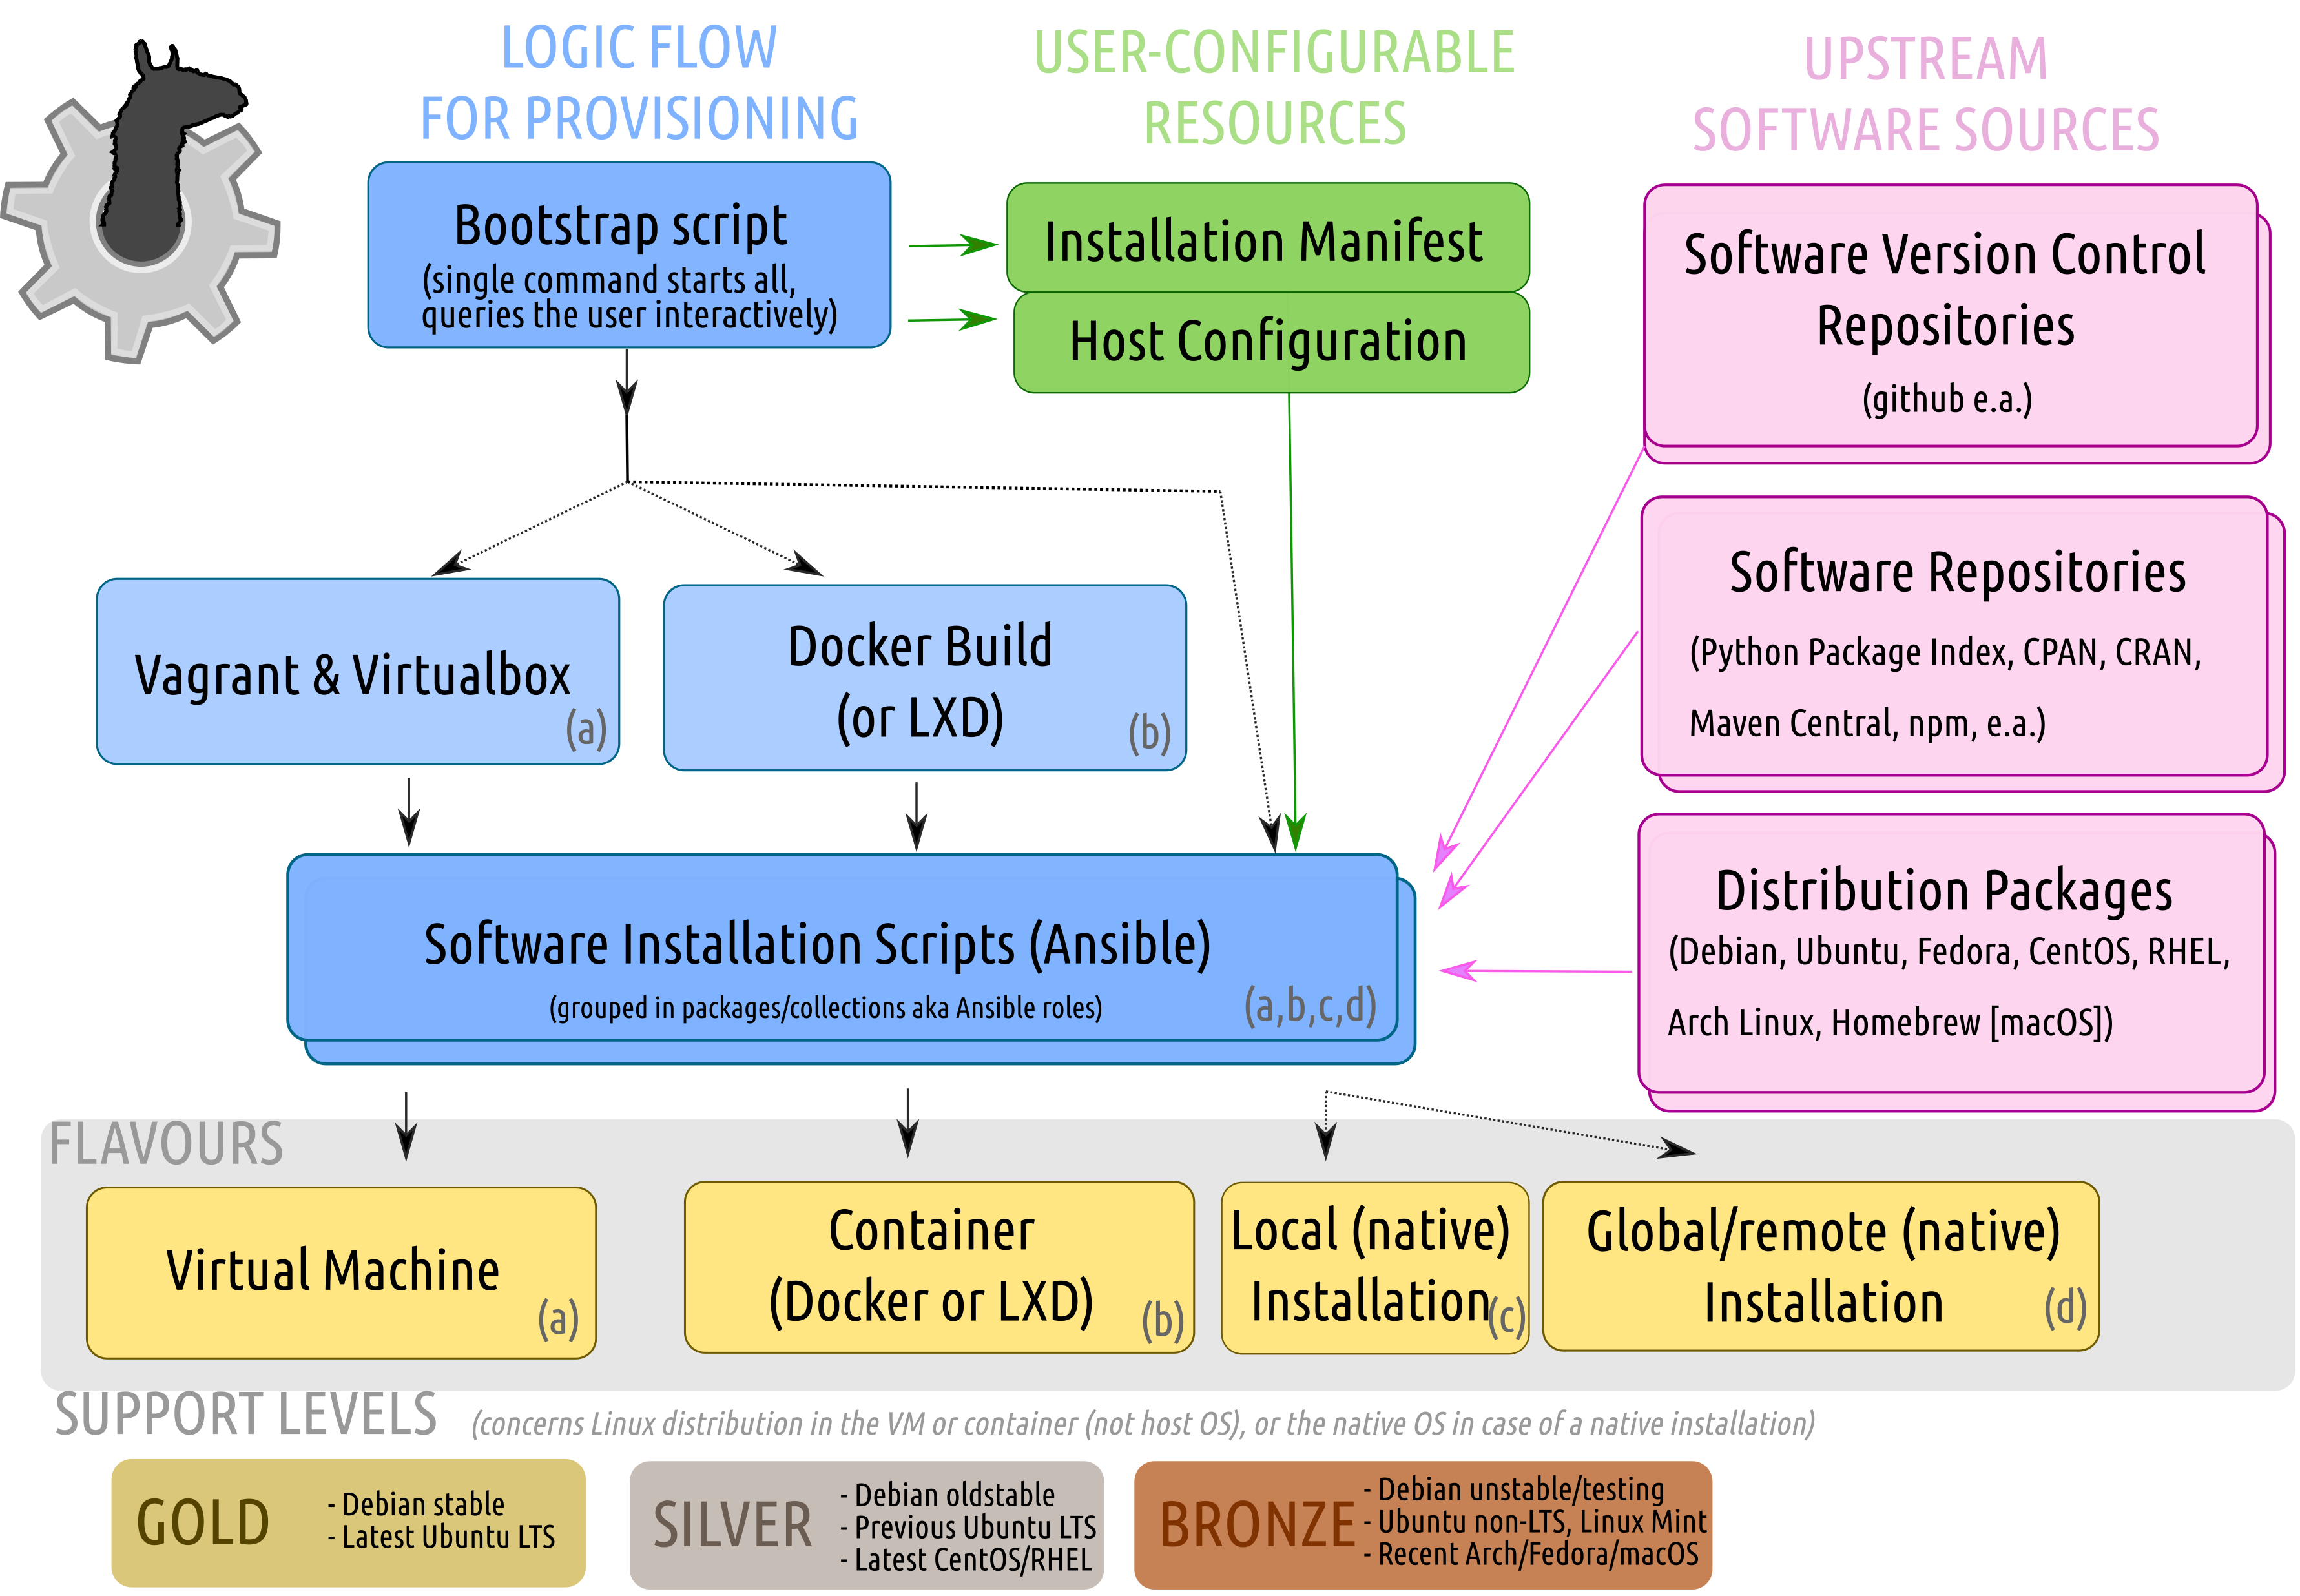
\includegraphics[width=135.0mm]{architecture.png}
\end{center}
\caption{\footnotesize{A schematic representation of the LaMachine architecture}}
\label{fig:arch}
\end{figure}

LaMachine also aims to harmonise the metadata of all installed software, by converting metadata from upstream
repositories, i.e. the repositories where tool providers deposit their software, to a common standard called CodeMeta
\footnote{\url{https://codemeta.github.io/}, described in JSON-LD} \cite{codemeta,codemetar} where possible, or
encouraging software developers to provide their codemeta metadata inside their source code repositories and using
that directly. This in turn enables other tools to do proper service discovery and provenance logging.

Leveraging this metadata, LaMachine comes with a webserver that offers a portal website with
access and overview of all installed tools, including web services and web applications. It also comes with a
Jupyter Lab\footnote{\url{https://jupyter.org/}} environment which provides a web-based Integrated Development
Environment (IDE) for scripting in Python and R, web-based terminal access, and so-called \emph{notebooks} which mix
text, code and data output and have gained great popularity in data science community nowadays.



\section{Software}

LaMachine exists since May 2015 and has been used extensively ever since by numerous users, in 2018 version 2 was
released which was a significant rewrite. LaMachine was initially conceived as the primary means of distribution of the
software stack developed at CLST, Radboud University Nijmegen. It therefore includes a lot of our software.  A full list
of included software goes beyond the scope of this overview; we will merely mention some CLARIN-NL/CLARIAH-funded tools:
ucto (a tokeniser), Frog (an NLP suite for Dutch), FoLiA (Format for Linguistic Annotation, with assorted tools), FLAT
(a web-based linguistic Annotation tool), PICCL (an OCR and post-OCR correction pipeline) and CLAM. However, this
project is not limited to one research group and is open to participation by other software providers, especially those
also in CLARIAH and the upcoming CLARIAH PLUS project. We already include some relevant software by other CLARIAH
partners. Moreover, LaMachine incorporates a large number of renowned tools by external international parties, offering
most notably a mature Python environment with renowned scientific modules such as scipy, numpy, scikit-learn,
matplotlib, nltk, spacy, pytorch, keras, gensim, tensorflow, and many others, but also R, Java and tools such as
Stanford CoreNLP and Kaldi.

\section{Case study}\label{sec-case}

We participated in a small Dutch national project titled \emph{`` Text mining for Inspection: an exploratory study on automatic analysis of health care complaints''} \footnote{project website:
\url{https://www.zonmw.nl/nl/onderzoek-resultaten/kwaliteit-van-zorg/programmas/project-detail/effectief-toezicht/tekstmining-in-het-toezicht-een-exploratieve-studie-naar-de-automatische-verwerking-van-klachten-in/}.
} led by IQhealthcare\footnote{\url{http://www.iqhealthcare.nl/nl/}}, the scientific centre for healthcare quality of RadboudUMC hospital.
This project took place at the Dutch Health Inspectorate and aimed to apply text mining techniques to health care
complaints that have been registered at the national contact point for health care (Landelijk Meldpunt
Zorg\footnote{\url{https://www.landelijkmeldpuntzorg.nl}})
We investigated the usefulness of text mining to categorise and cluster complaints, to automatically determine the
severity of incoming complaints, to extract patterns  and to identify risk cases. This project turned out to be a good
test case of the applicability and usefulness of LaMachine as a standalone research environment.
As the complaint data is highly sensitive, it could not leave the secure servers of the health inspectorate and was
stored in an environment without internet access. We needed to bring the software to the data via a shared folder.

We used a virtual machine (VM) image of LaMachine and we ran this 64-bits Linux-based VM inside another
VM with Windows Server 2012, provided to us by the health inspectorate for this project, in which we did have administrative
rights but no internet access. In terms of hardware we ran on a machine with 8 cores and  32GB internal memory available.
%using VirtualBox and Vagrnt on the Windows VM
LaMachine provided a fully functional research environment and we ran all our experiments within LaMachine. We interacted with LaMachine both through the command line, which offers a standard
shell and enables access to all lower-level tools and programming languages; and through the (offline) webbrowser to use
the Jupyter Notebook environment.

LaMachine comes with some simple data sharing facilities that allowed us to access the sensitive complaint data via a
single shared dataspace between host and the VM. Extensive data search and management functions are deliberately beyond the scope of LaMachine, and left to more high-level tooling.

We used many of the available tools in LaMachine within this project: Frog for linguistic annotation of the textual
content of the complaint and the scikit-learn Python package for classification, T-scan for feature extraction in the form of text characteristics and colibri-core for n-gram analysis.

%het doel van deze studie is om automatische tekstanalysetechnieken (tekstmining) toe te passen op de klachten die bij het Landelijk Meldpunt Zorg binnenkomen. Zo hopen we eventuele trends en patronen te vinden die meer inzicht geven in de aard en de relevantie van de klachten. De verwachting is om zo potentiële risicogevallen te ontdekken die op basis van de behandeling van individuele klachten nog niet waren gesignaleerd.

\section{Conclusion \& Future work}

The recent release of LaMachine v2, which constituted a full rewrite, has opened up LaMachine to outside
contribution. Contributor documentation has been written, and at this stage, we greatly welcome external participants
to join in. Use cases as the example in section \ref{sec-case} contribute to thorough testing and running of LaMachine in less ideal circumstances such as nested VM constructions and offline usage.

Aside from the incorporation of new relevant software, the main objectives for the future are to provide
greater \emph{interoperability} between the included tools through better \emph{high-level interfaces} for the
researcher. We see this as a bottom-up process and have now established a firm foundation to build upon. Note that such
proposed interfaces, including the current portal application in LaMachine, are always considered separate independent
software projects, which may be deployed by/in/for LaMachine, but also in other contexts. LaMachine remains `just'
a software distribution at heart.

Development of LaMachine presently takes place in collaboration with the CLARIAH WP3 Virtual Research Environment (VRE)
project\footnote{\url{https://github.com/meertensinstituut/clariah-wp3-vre}}, which has higher ambitions in
accommodating the researcher and connectivity of data and services, and transcends also those of the CLARIN Language
Resource Switchboard~\cite{switchboard}. An important part of our future focus will therefore be on interoperability
with the higher-level tools emerging from the VRE efforts, but also with other parts of the CLARIN infrastructure;
single-sign on authentication being a notable example here.

\section*{Acknowledgement}

This research was funded by NWO CLARIN-NL, CLARIAH and the ZonMw project {\it Tekstmining in het toezicht: een exploratieve studie naar de automatische verwerking van klachten ingediend bij het Landelijk Meldpunt Zorg}, project number 516004614. We thank all project partners: the Dutch Health Inspectorate, IQhealthcare, and Tim Voets for their valuable contributions and help in the ZonMw project.


\bibliography{lamachine}



\end{document}

